\documentclass[12pt]{article}

\usepackage{dsfont}
\usepackage{float}
\usepackage{amsmath}
\usepackage{graphicx}
\usepackage{enumitem}
\usepackage[margin=1.50in]{geometry}
\usepackage[font=footnotesize]{caption}

\usepackage{bm}
\newcommand{\m}[1]{\mathbf{\bm{#1}}}
\newcommand{\R}{I\hspace{-4.4pt}R}


\usepackage{natbib}
\bibpunct{(}{)}{;}{a}{}{,}

\begin{document}

\begin{LARGE}
\noindent Dirichlet process mixture model on \\ Hopkinson-bar experiments
\end{LARGE}
\bigskip

\noindent Mickey Warner

\noindent AMS 241

\section{Introduction}

Hopkinson-bar (or Split-Hopkinson pressure bar) experiments are compression tests performed on small (e.g. 6.35mm diameter) samples of materials. The material undergoes a deformation which is measured by a strain-stress ($\epsilon$-$\sigma$) response. Strain measures changes in the length of the material, and stress measures changes in the cross-sectional area. A single experiment yields a strain-stress curve.

An experiment may fall within two classes of tests: quasi-static or dynamic. In quasi-static tests, the compression occurs very slowly, attempting to measure infinitesimal changes in the response. These are associated with low strain rates, $\dot\epsilon$. Dynamic tests occur at high strain rates and are characterized by higher volatility in the response curve.

Other variations of this experiment exist, but the data we will look at in this paper come from either quasi-static or dynamic tests. The data are of Hopkinson-bar tests performed on samples of tantalum by \cite{chen1996constitutive} (see figure \ref{data}), at various strain rates and initial temperatures.

The goal is to model these response curves so we can make accurate predictions for future experiments. The curves themselves (and consequently any predicted curve) may be fed into more complicated materials science models such as those involving 3-D printing. Materials models have been developed to capture the physics and behavior of Hopkinson-bar experiments. We will use a simplified version of a particular model, the Johnson-Cook model, in conjunction with a Dirichlet process mixture model, as our statistical model.

In section 2, we discuss some of the ideas used in modeling these kinds of experiments, from both materials science and statistics perspectives. We discuss Dirichlet process mixture models in section 3 and provide an example of its usage to a simulated data set in section 4. In section 5 we analyze the Hopkinson-bar tests from \cite{chen1996constitutive}. We conclude in section 6 with a discussion.

\begin{figure}[H]
\begin{center}
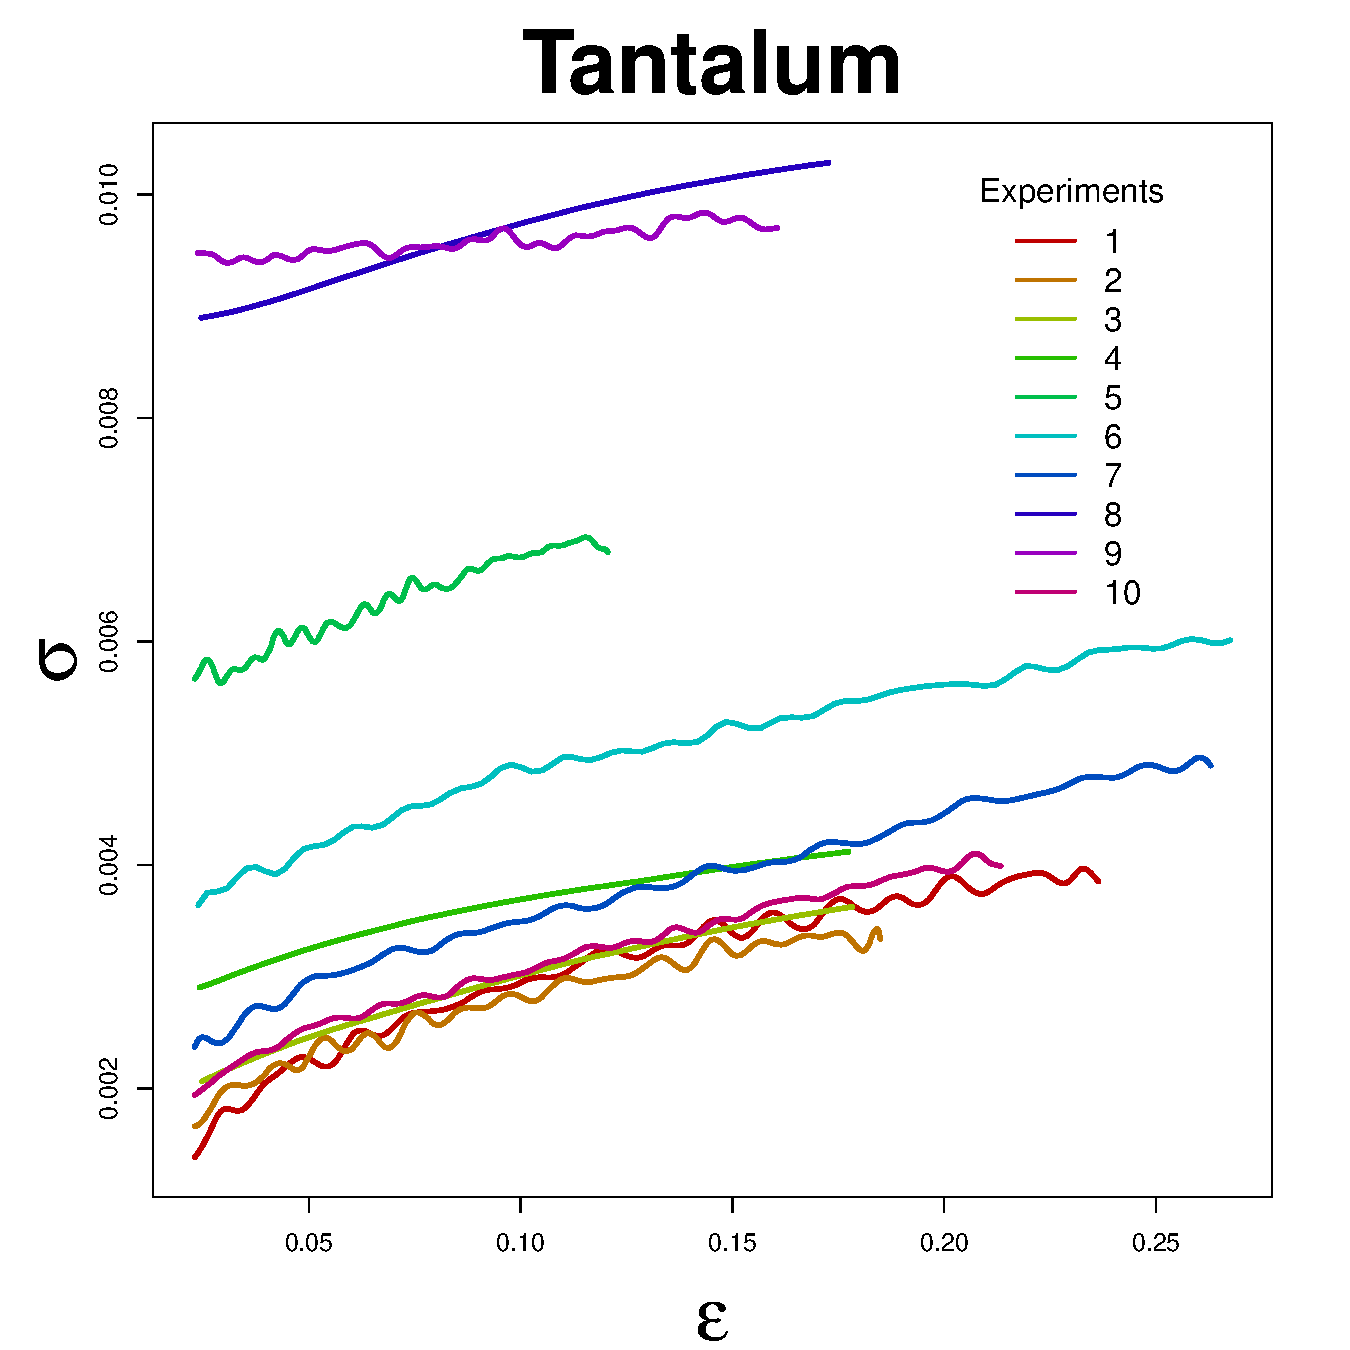
\includegraphics[scale=0.40]{../figs/ta_all_data.pdf}
\caption{Strain-stress response from ten experiments at various strain rates and temperatures.}
\label{data}
\end{center}
\end{figure}

\section{Brief review of current approaches}

Perhaps the simplest materials model that attempts to model the stress $\sigma$ is the Johnson-Cook model:
\begin{align}
\m{\sigma}(\m{x}, \m{\theta}) = (A+B\epsilon_p^n)(1+C\log\dot\epsilon)(1-T^m)
\label{jc}
\end{align}
where $\m{x}$ encodes the plastic strain $\epsilon_p$ (the $x$-axis in figure \ref{data}), strain rate $\dot\epsilon$, and initial temperature $T$ for a specific experiment, and $\m{\theta}=(A,B,n,C,m)$ is the vector of parameters to be estimated. Other models exist that may have more parameters, and hence better predictive capabilities, but model (\ref{jc}) provides us with a convenient starting point.

A typical approach in the materials science community is to assume a common $\m{\theta}$ among all experiments and then minimize some goodness-of-fit function. The minimization may be done by optimizing one parameter at a time, holding some parameters fixed (for more complicated models), or even by looking at a graph. We would at least prefer a systematic method of estimating the parameters.

A challenge for any materials model is the potential lack in accurately accounting for all of the necessary physics in the experimental procedure. If a key component is missing, predictions made at untried experimental settings may fail. If too many terms are added, we run the risk of overfitting.

\cite{fugate2005hierarchical} fit a hierarchical Bayesian model to Hopkinson-bar experiments where the mean curve is given by a materials model such as (\ref{jc}). By assuming each experiment has its own $\m{\theta}_i$, the authors found that the added flexible increased the predictive power of the statistical model. A model with common $\m{\theta}$ yielded predictive uncertainty that was too conservative. In the hierarchical setting, the mean predictive curve for a new experiment was more accurate, but the predictive variance necessarily increased.

A parametric assumption made by \cite{fugate2005hierarchical} is that the population distribution for the $\m{\theta}_i$'s is (truncated) multivariate normal. For data sets or materials models where the random effects $\m{\theta}_i$ do not come from a normal distribution, predictions based on this hierarchical model do very poorly.

\section{Dirichlet process mixture models}

Before introducing the Dirichlet process mixture (DPM) model, we write out the hierarchical model used by \cite{fugate2005hierarchical}. For experiments $i=1,\ldots,n$, we have a vector of measured stresses, denoted $\m{y}_i$, modeled as
\begin{align}
\m{y}_i|\m{x}_i,\m{\theta}_i &\overset{ind}\sim N_{k_i}(\m{y}_i|\m{\sigma}(\m{x}_i,\m{\theta}_i),\tau^2\m{I}_{k_i}) \label{para} \\
\m{\theta}_i|\m{\mu}, \m{\Sigma} &\overset{iid}\sim N_p(\m{\theta}_i|\m{\mu},\m{\Sigma})\times\mathds{1}(\m{\theta}_i\in C) \label{para_rand} \\
\m{\mu} &\sim N_p(\m{\mu}|\m{m}, \m{S})\times\mathds{1}(\m{\mu}\in C) \nonumber \\
\m{\Sigma} &\sim IW(\m{\Sigma}|\m{V}, d) \nonumber \\
\tau^2 &\sim IG(\tau^2|a_{\tau^2}, b_{\tau^2}) \nonumber
\end{align}
where $\m{x}_i=(\m{\epsilon}_{pi},\dot\epsilon_i,T_i)$ is a contains the plastic strains $\m{\epsilon}_{pi}$, strain rate $\dot\epsilon_i$, and initial temperature $T_i$ for each $i$, $\m{\sigma}(\cdot)$ is given in eq. (\ref{jc}), $\m{m}, \m{S}, \m{V}, d, a_{\tau^2}, b_{\tau^2}$ are known, and $C\subseteq \R^p$ is a set of constraints specified by the materials model. The function $\mathds{1}(x \in A)$ returns $1$ if $x$ is an element of the set $A$ and $0$ otherwise. We will call this model the parametric model.

Depending on the materials model, the normal distribution assumption (\ref{para_rand}) for the random effects may be inappropriate. Therefore, we may wish to be more flexible than this specification.

The Dirichlet process mixture model assumes a non-parametric prior on the distribution of random effects. We replace (\ref{para_rand}) with
\begin{align}
\m{\theta}_i|G &\overset{iid}\sim G \nonumber \\
G|\alpha, \m{\mu}, \m{\Sigma} &\sim DP(\alpha, G_0=N_p(\m{\theta}_i|\m{\mu},\m{\Sigma})\times\mathds{1}(\m{\theta}_i\in C)) \nonumber
\end{align}
and keep all else from the parametric model the same.

The posterior distributions for $\m{\mu}$, $\m{\Sigma}$, and $\tau^2$ in both models can be updating using Gibbs steps. Since $\m{\sigma}(\cdot)$ is non-linear, updating $\m{\theta}_i$ in both models is made with Metropolis steps. In the parametric model, the step should be straight-forward. In the DPM model, we update $\m{\theta}_i$ after integrating out the infinite-dimensional parameter $G$. Algorithm 6 by \cite{neal2000markov} is used for these updates.

\section{Simulation example}

To illustrate some practical differences between the parametric and the DPM models, we consider a toy example (see figure \ref{toy}). We generate $i=1,\ldots,n=100$ curves, each denoted by $\m{y}_i$, with random intercepts and linear and quadratic coefficients, according to
\begin{align*}
\m{y}_i &= \beta_{i0}\m{1}_{k_i} + \beta_{i1}\m{x}_i + \beta_{i2}\m{x}_i^2 + \m{\epsilon}_i \\
\m{\epsilon}_i &\overset{iid}\sim N(0, 0.05^2\m{I}_{k_i}) \\
\beta_{i0} &\overset{iid}\sim N(3, 0.3^2) \\
\beta_{i1} &\overset{iid}\sim N(1.5, 0.1^2) \\
\beta_{i2} &\overset{iid}\sim 0.5\delta_0(\cdot) + 0.5N(-1, 0.1^2)
\end{align*}
where $\m{x}_1=\cdots=\m{x}_n=(-0.5,\ldots,2)^\top$ are vectors of $k_i=10$ equally spaced points and $\m{x}^2$ denotes element-wise squaring. The vector $\m{x}_i$ should not be thought of only as covariates, but rather the locations where measurements were made, say for repeated measures or functional data.

We fit the simulated data to both the parametric and DPM models, where $\m{\sigma}(\cdot)$ is replaced with the polynomial $p(\m{x}, \m{\beta})=\beta_0\m{1}_{k_i}+\beta_1\m{x}+\beta_2\m{x}^2$. So we are assuming that every coefficient in the linear model is a random effect.

\begin{figure}
\begin{center}
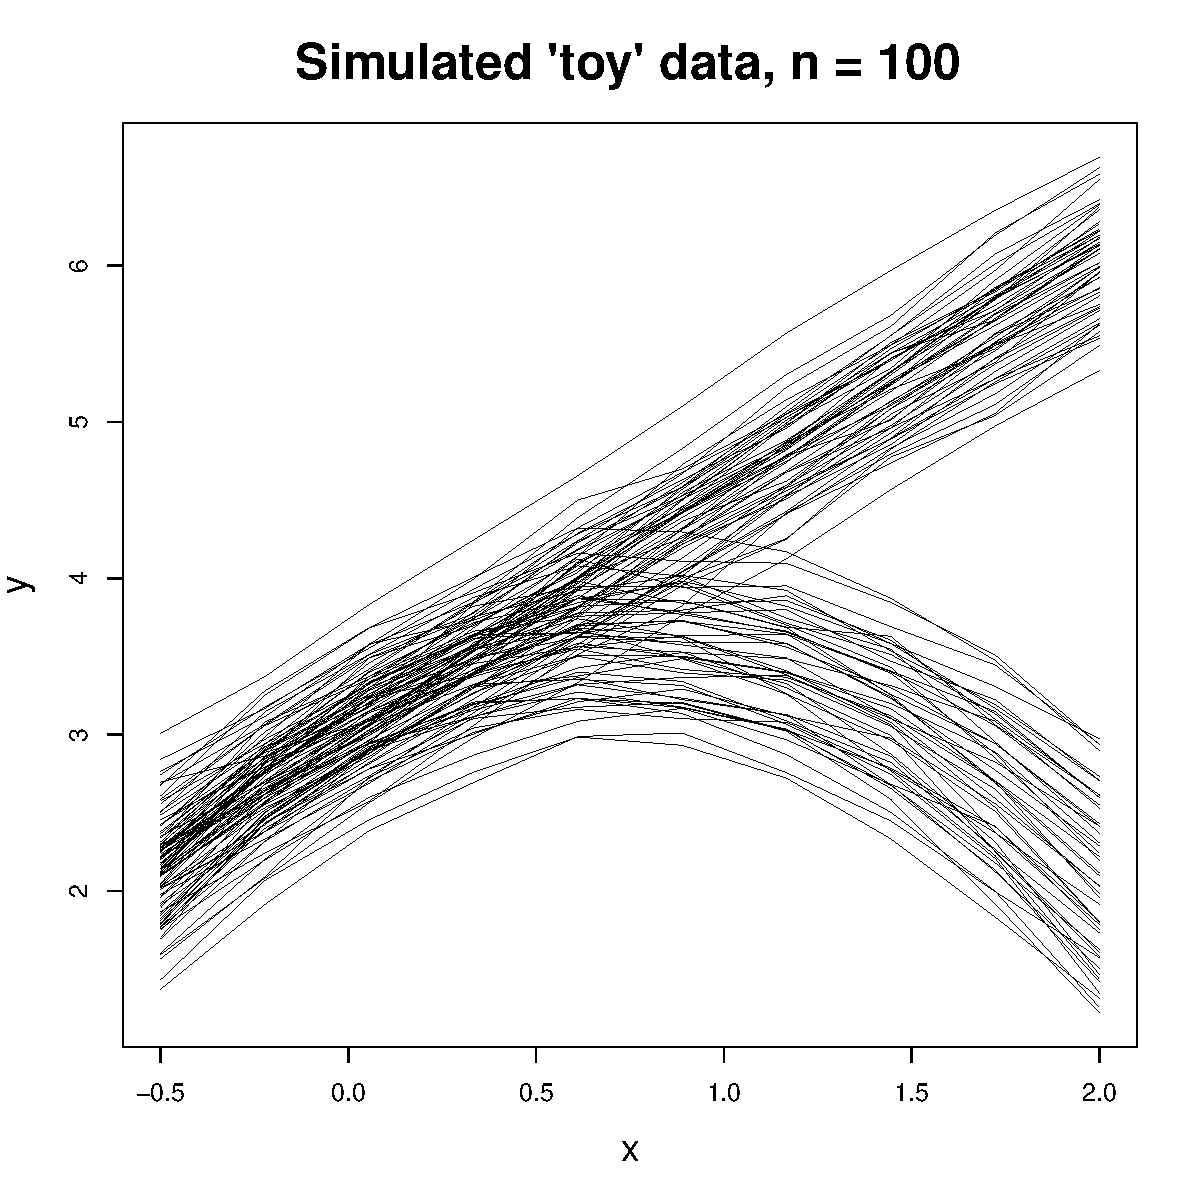
\includegraphics[scale=0.37]{../figs/toy_data.pdf}
\caption{Simulated data set.}
\label{toy}
\end{center}
\end{figure}

\begin{figure}
\begin{center}
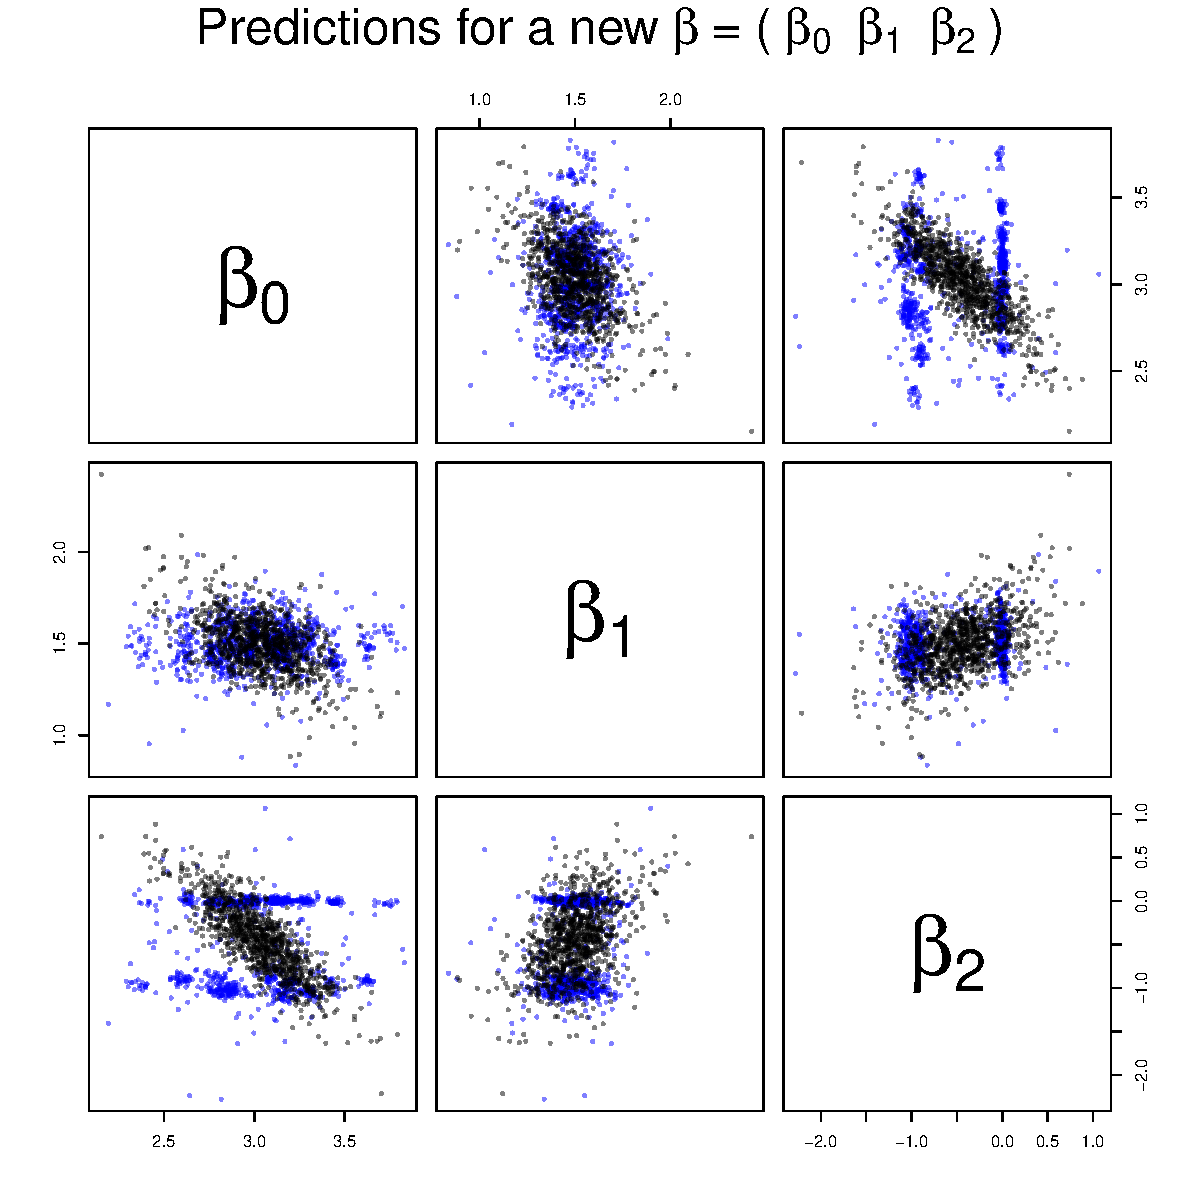
\includegraphics[scale=0.45]{../figs/toy_theta_0.pdf}
\caption{Posterior predictive distribution of a new random effect $\m{\beta}_0$. Black: parametric model. Blue: DPM model.}
\label{toy_theta}
\end{center}
\end{figure}

\begin{figure}
\begin{center}
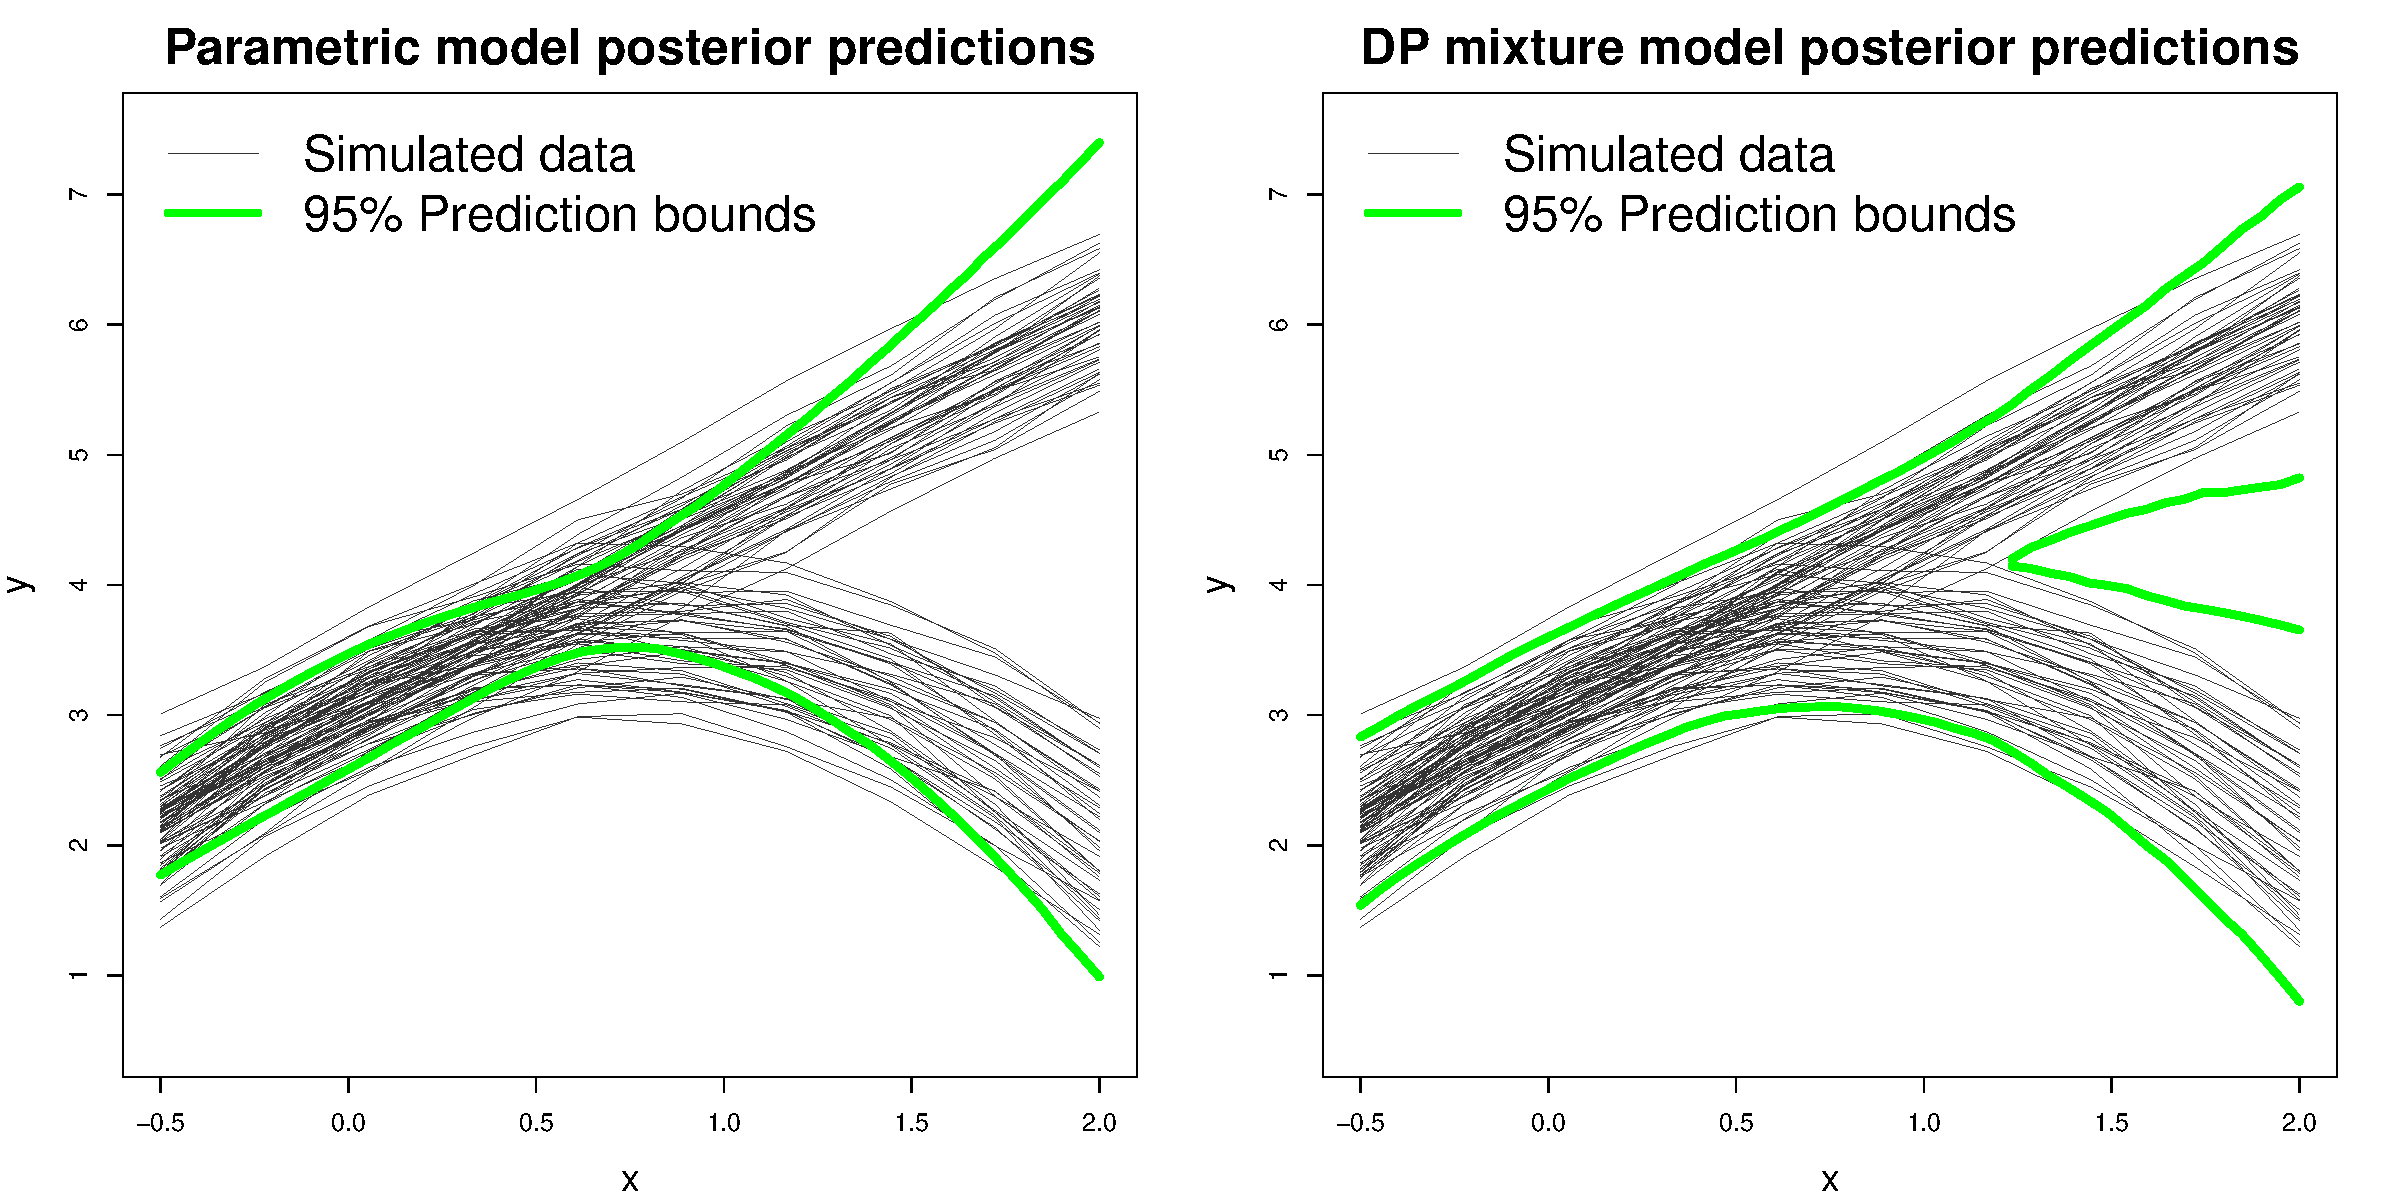
\includegraphics[scale=0.34]{../figs/toy_y_0.pdf}
\caption{The posterior predictive distribution of a new observation $\m{y}_0$ based on $\m{\beta}_0$ shown with the green 95\% prediction bounds. Left: parametric model. Right: DPM model.}
\label{toy_y}
\end{center}
\end{figure}

Posterior predictions for each model are shown in figures \ref{toy_theta} and \ref{toy_y}. Even though both models estimated the random effects $\m{\beta}_i$ for each observation to be nearly the same, we can see a clear difference in the predictions. Figure \ref{toy_theta} shows a pairs plot for the predictive distribution for a new random effect $\m{\beta}_0$, and \ref{toy_y} shows a 95\% predictive region for a new observation $\m{y}_0$. Notice that the parametric model produces a normal distribution for $\m{\beta}_0$, while the DPM more correctly captures the bimodality in the quadratic term. In figure \ref{toy_y} we observe that the parametric model is unable to capture the distinction between the lines and the parabolas in the data. However, the DPM model is capable of doing just that since the non-parametric prior allows for flexible random effects distributions.

\section{Analysis of the Hopkinson-bar experiments}

We now turn our attention back to the Hopkinson-bar experiments of \cite{chen1996constitutive} (see figure \ref{data}). A previous analysis fit the parametric modeled described in section 3 and used the Johnson-Cook model (\ref{jc}) as the mean of the curves. It was noted that the parametric model failed to produce adequate predictions: it was clear that the population distribution for the random effects was not normal.

\begin{figure}
\begin{center}
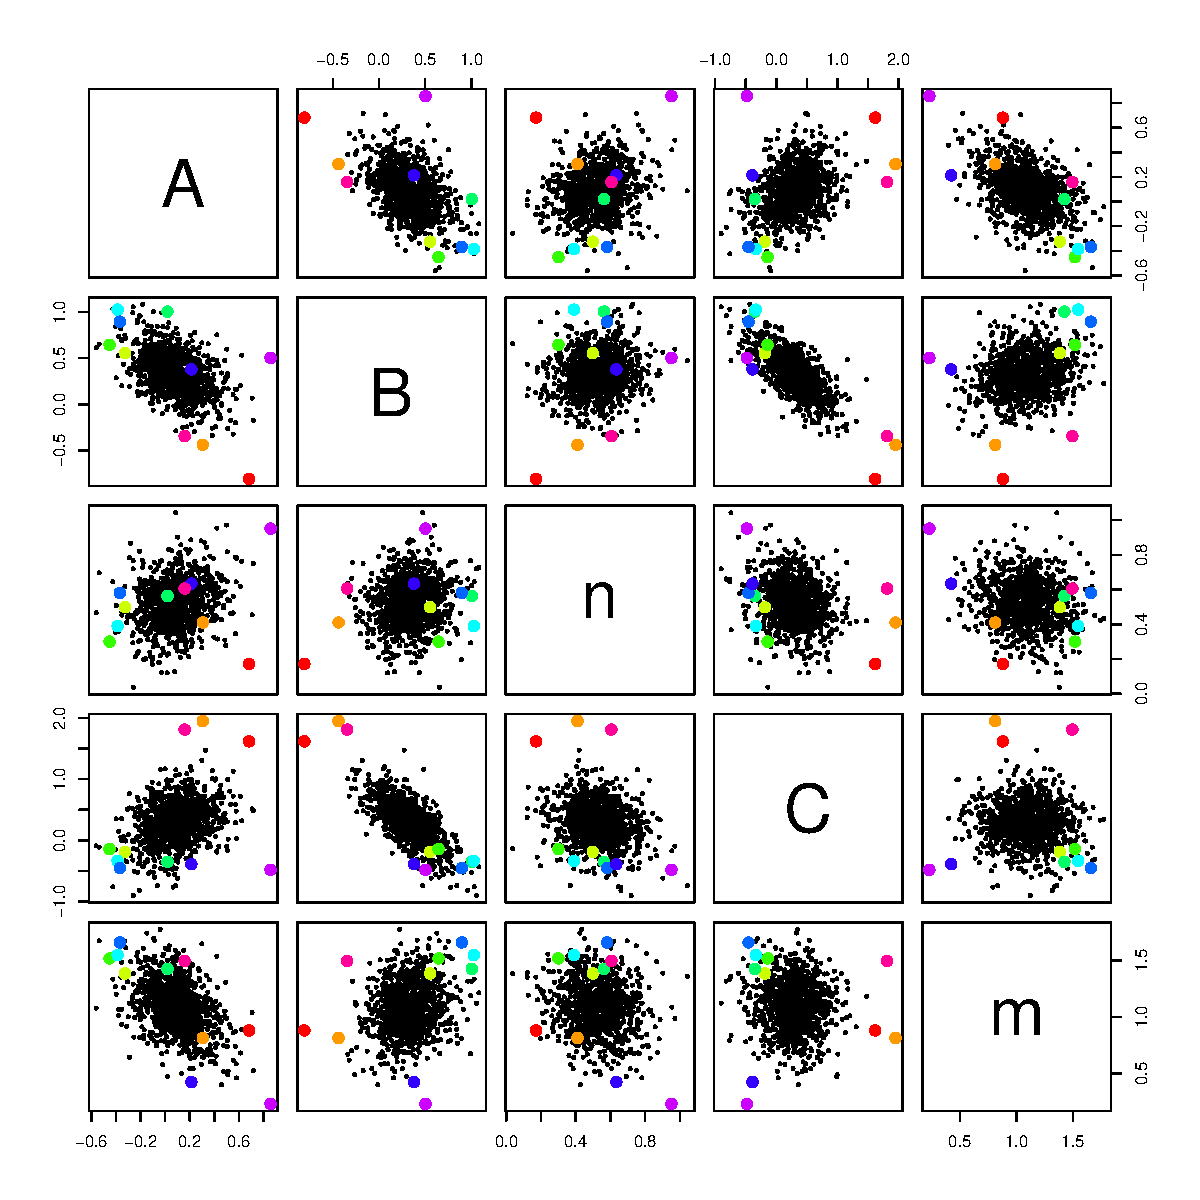
\includegraphics[scale=0.43]{../figs/ms_clusters.pdf}
\caption{Each two-way dot plots of baseline mean $\m{\mu}$ (black dots) and the means of each random effect (colored dots).}
\label{ms_clusters}
\end{center}
\end{figure}

\begin{figure}
\begin{center}
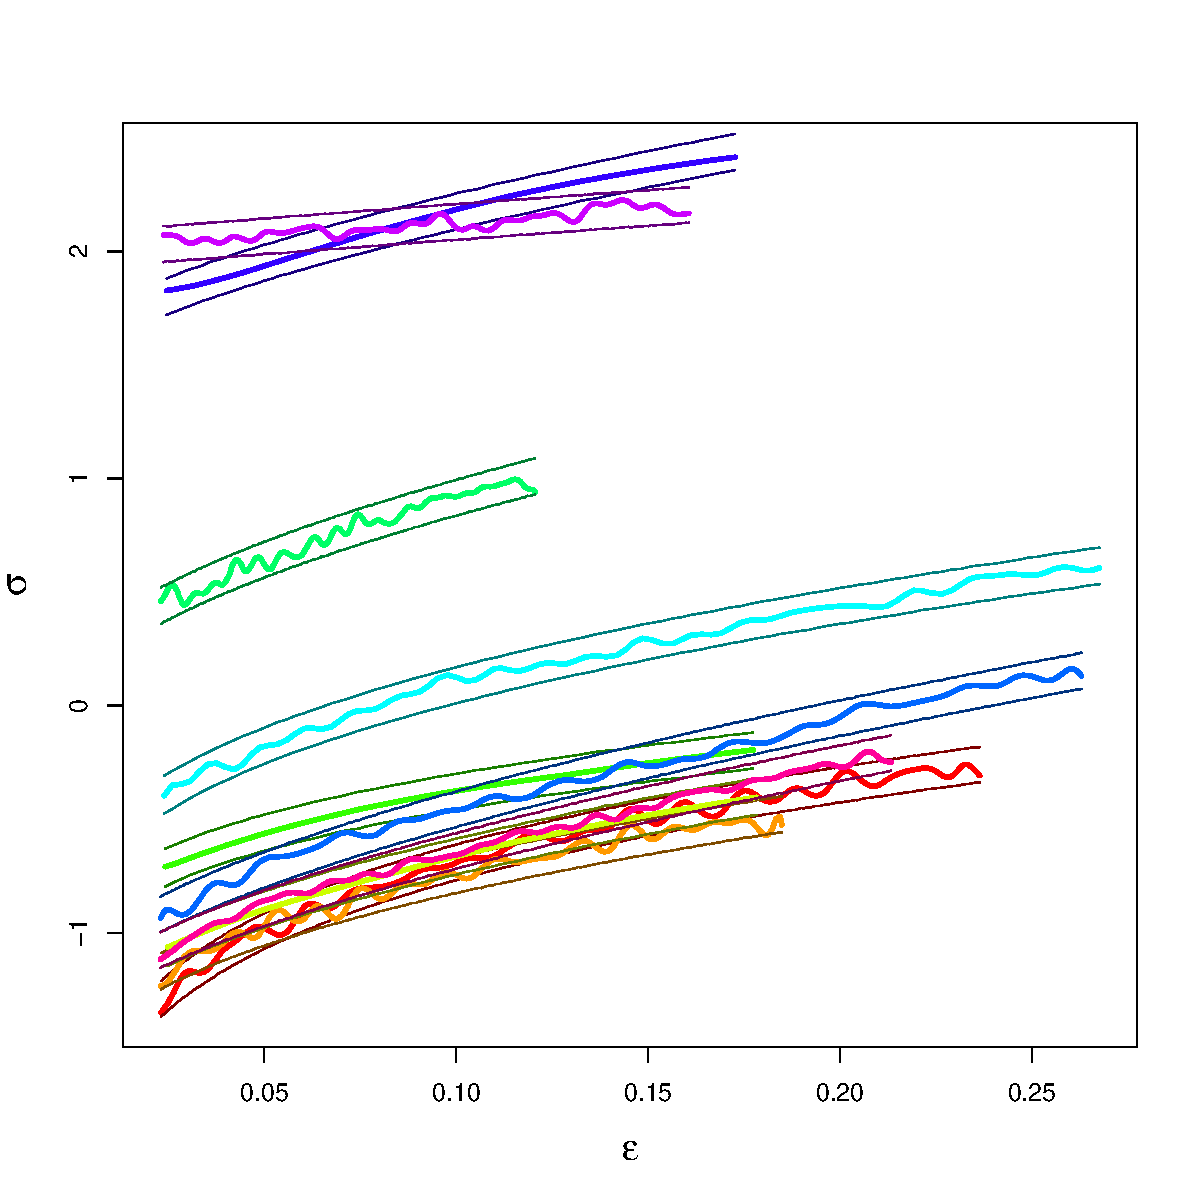
\includegraphics[scale=0.39]{../figs/ms_predsA.pdf}
\caption{95\% prediction bounds for each observation using its estimated random effect distribution.}
\label{ms_y}
\end{center}
\end{figure}

The Dirichlet process mixture model of section 3 was subsequently fit to the data, with the hope that the non-parametric assumption would yield better results. To our dismay, poor predictions were also produced by this model. Figure \ref{ms_clusters} shows bivariate projections of the distribution for the baseline mean $\m{\mu}$ (in black) and the means of the random effects $\m{\theta}_i$ (in colors). If we know the random effect for a particular experiment, we can achieve very accurate predictions (as in figure \ref{ms_y}). However, these are meaningless in predicting a new experiment. Predictions based on a new $\m{\theta}_0$ were so outrageously inaccurate, with such high variance, that showing them would be pointless.

Though the DPM model allows for a more flexible population distribution, the problem with predictions are due to the Johnson-Cook model being very sensitive to a change in parameters. Consider again figure \ref{ms_clusters}. The colored dots correspond to the mean of posterior random effects for each observation. The figure does not show it, but the variance around each of these points is very small. So when predicting a new experiment, with a given strain rate and temperature, the ``correct'' random effect to choose from will only be selected a few times and anything away from this ``correct'' value would produce highly unrealistic predictions. In this sense, the random effects are \emph{too} unique across experiments and do not share enough information.

\section{Discussion}

In this paper we fit a Dirichlet process mixture model to Hopkinson-bar experiments. At particular strain rates and temperatures, these experiments result in strain-stress curves. Materials models such as the Johnson-Cook model (\ref{jc}) attempt to model the curves. Early attempts at fitting the materials models showed that a common parameter vector may not be optimal, hence a hierarchical approach has been taken.

Depending on the choice of materials model, the multivariate normal assumption on the population distribution may be suspect. To address this, we assumed a non-parametric prior on the population distribution. However, similar difficulties existed in both the parametric setting and the non-parametric setting. Predicting new experiments still faced the challenge of an overly sensitive materials model.

Since the Johnson-Cook model is known to be overly simplistic, we do not expect this kind of poor predictive behavior to be found when using another model such as mechanical threshold stress. The goal here was to identify potential weaknesses in the DPM model and in the materials model. Had the materials model been correctly specified, when making predictions we would have drawn $\m{\theta}$s too frequently which yield unrealistic results. A possible next step could be to use a new covariate $\m{x}^*$ to decide $\m{\theta}_i$ to draw from. I suspect that if $\m{x}^*$ is near the $\m{x}_i$ of an experiment used to fit the model, drawing from that experiments $\m{\theta}_i$ may produce better results. Perhaps this may be done by making $\m{\mu}$ a function of the covariates.

\bibliography{refs}
\bibliographystyle{asa}


\end{document}
